\documentclass[border=6pt]{standalone}
\usepackage{tikz}
\usetikzlibrary{arrows.meta,positioning,calc,shapes.geometric,fit,backgrounds,patterns,matrix,decorations.pathreplacing}
\begin{document}
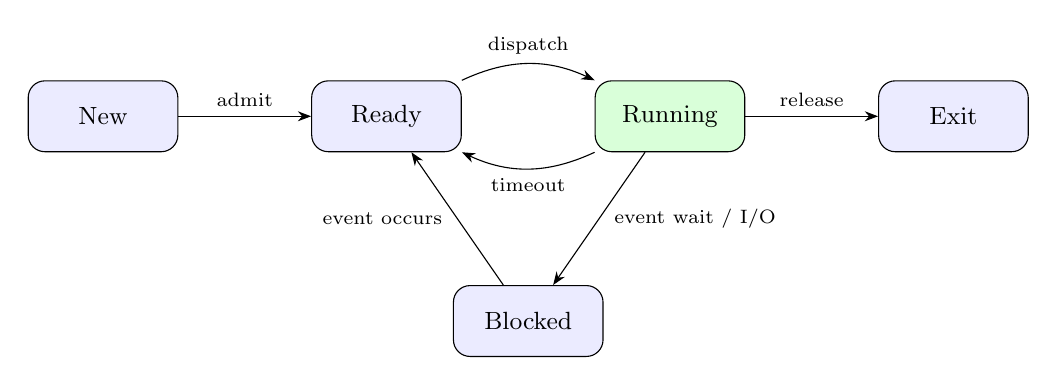
\begin{tikzpicture}[>=Stealth,font=\small]
\tikzstyle{st}=[draw,rounded corners=6pt,minimum width=1.9cm,minimum height=0.9cm,fill=blue!8]
\node[st] (n) at (0,0) {New};
\node[st] (r) at (3.6,0) {Ready};
\node[st,fill=green!15] (u) at (7.2,0) {Running};
\node[st] (e) at (10.8,0) {Exit};
\node[st] (b) at (5.4,-2.6) {Blocked};
\draw[->] (n) -- node[above,font=\scriptsize]{admit} (r);
\draw[->] (r.north east) to[bend left=25] node[above,font=\scriptsize]{dispatch} (u.north west);
\draw[->] (u.south west) to[bend left=25] node[below,font=\scriptsize]{timeout} (r.south east);
\draw[->] (u) -- node[above,font=\scriptsize]{release} (e);
\draw[->] (u) -- node[right,font=\scriptsize,xshift=2pt]{event wait / I/O} (b);
\draw[->] (b) -- node[left,font=\scriptsize,xshift=-2pt]{event occurs} (r);
\end{tikzpicture}
\end{document}
